\documentclass{beamer}
\usetheme{metropolis}           % Use metropolis theme

\usepackage[T2A]{fontenc}
\usepackage[utf8]{inputenc}
\usepackage[english, main=russian]{babel}

\usepackage{listingsutf8}
\usepackage[ruled]{algorithm}
\usepackage{algorithmicx}
\usepackage[noend]{algpseudocode}
\usepackage{amsmath}
\usepackage{caption} 
\usepackage{graphicx}
\usepackage{subcaption}
\usepackage{float}

\floatname{algorithm}{Листинг}
\renewcommand{\algorithmname}{Листинг}

\title{Классификация графиков вероятностных распределений методами компьютерного зрения}
\date{\today}
\author{Утебаева Милена}
\author[me]{Выполнила: Утебаева Милена ИУ9-51Б\\[1mm]Руководитель: Цалкович П.А.}
% \thanks
% \institute{МГТУ им. Н.Э. Баумана}
\begin{document}
\maketitle

\begin{frame}{Цели и задачи}
  \metroset{block=fill}
	\begin{alertblock}{Цель}
		Разработать модель машинного обучения для распознавания графиков вероятностных распределений, сравнить различные преобразования изображений, направленные на повышение точности прогноза.
	\end{alertblock}
	\begin{alertblock}{Задачи}
    
		\begin{itemize}
			\item Изучить методы компьютерного зрения;
			\item Подготовить данные для обучения нейронных сетей;
			\item Реализовать несколько свёрточных нейронных сетей, обучить их на изображениях с разным типом преобразований;
			\item Проанализировать и сравнить между собой получившиеся модели, выбрать наилучшую по метрикам качества.
		\end{itemize}
	\end{alertblock}
\end{frame}



\begin{frame}{Машинное обучение}

	\alert{Машинное обучение} -- раздел информатики, который посвящён созданию алгоритмов, опирающихся на набор данных о каком-либо явлении. Данные могут быть различного происхождения: получены из окружающей среды, порождены другими алгоритмами или созданы вручную.



\end{frame}

\begin{frame}{Компьютерное зрение}

	\alert{Компьютерное зрение} -- направление машинного обучения, которое занимается исследованиями в области различного рода обработки изображений.

  \metroset{block=fill}
	\begin{alertblock}{Основные задачи компьютерного зрения}
		\begin{enumerate}
			\item Распознавание объектов на изображении
                \item Классификация объектов на изображении
			\item Сегментация изображений
			\item Стилизация изображений
		\end{enumerate}
	\end{alertblock}



\end{frame}

\begin{frame}{Свёрточная нейронная сеть}

	\alert{Свёрточная нейронная сеть} -- архитектура нейронной сети, позволяющая извлекать нетривиальные признаки из изображений. Своё название данная архитектура получила из-за наличия операции свёртки.



\end{frame}

\begin{frame}{Операция «свёртка»}

\begin{figure}[H]
		\centering
		\begin{minipage}[t]{.75\textwidth}
			\centering
			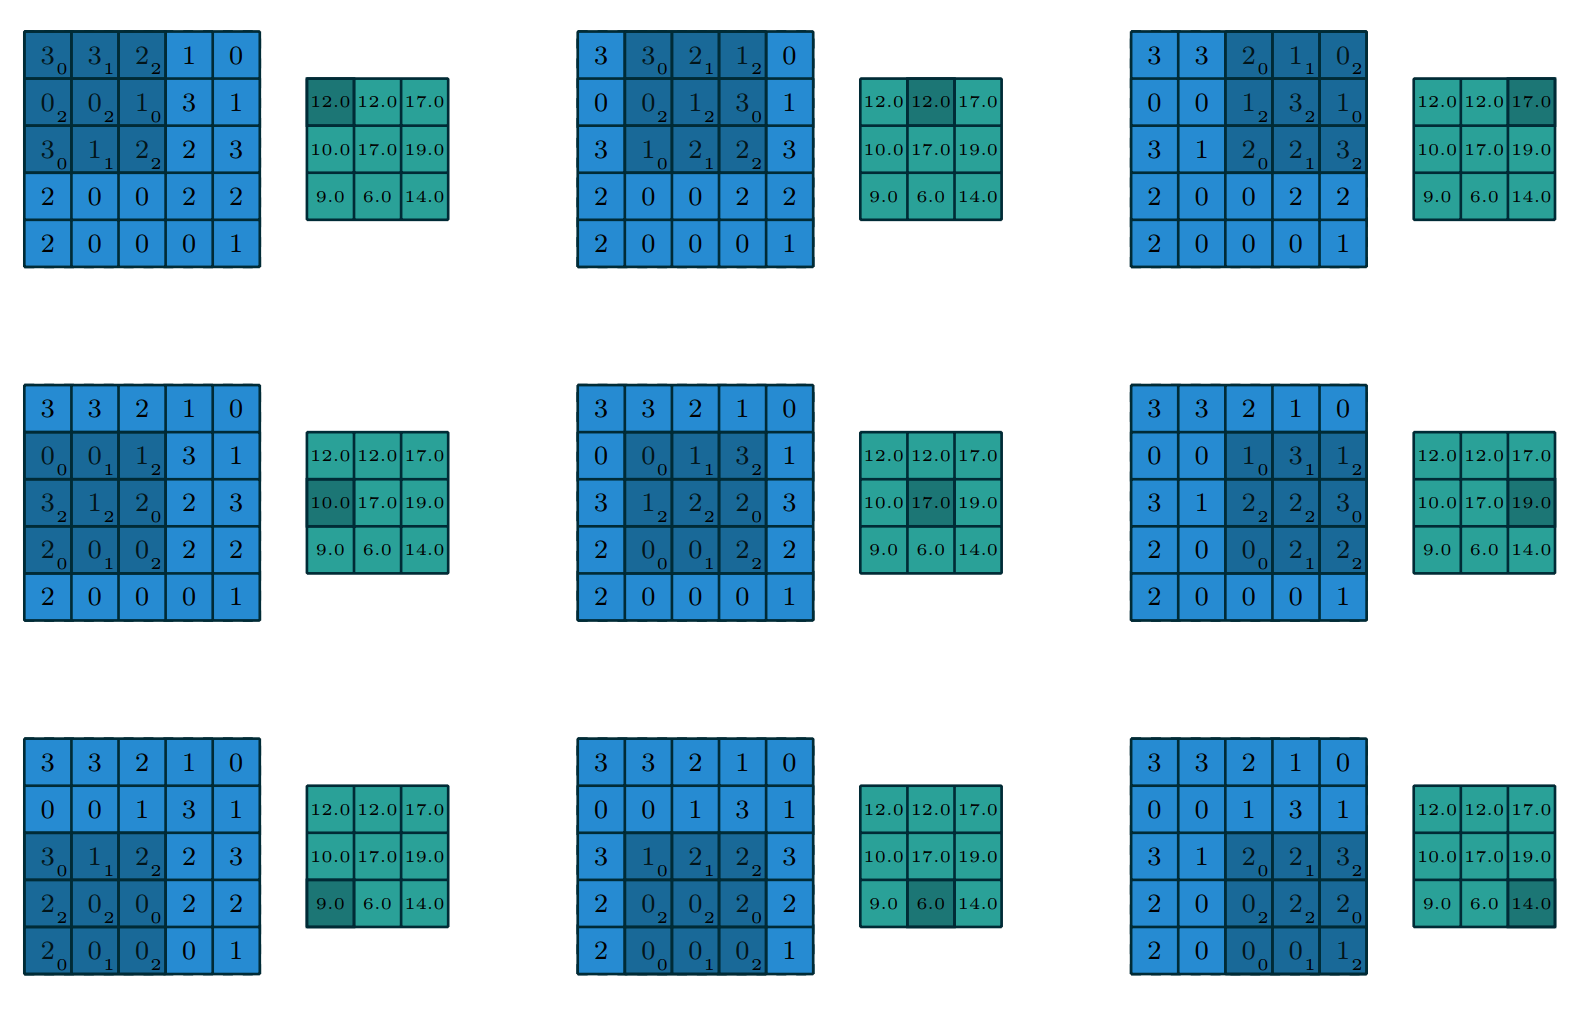
\includegraphics[width=\linewidth]{./img/svertka.png}
		\end{minipage}
		\caption{Пример процесса свёртки.}
	\end{figure}

\end{frame}

\begin{frame}{Тензорное представление изображений}

        \alert{Изображения} в контексте обработки алгоритмами компьютерного зрения являются упорядоченным набором пикселей. 

        \alert{Каждый пиксель} -- это вектор. Для чёрно-белых изображений он состоит из одного канала, а для цветных — из трёх: интенсивностей красного, зелёного и синего цветов.



\end{frame}

\begin{frame}{Преобразования над изображениями}
        \alert{Преобразование изображения} -- это набор определённых манипуляций, проводящихся над пикселями.

  \metroset{block=fill}
	\begin{alertblock}{Примеры преобразований над изображениями}
		\begin{enumerate}
			\item Изменение свойств изображения: яркости, контрастности, насыщенности
			\item Перспективное преобразование
			\item Поворот
		\end{enumerate}
	\end{alertblock}


\end{frame}

\begin{frame}{Пример изображений после преобразования}

	\begin{figure}[H]
	\centering
	\begin{minipage}[t]{.3\textwidth}
		\centering
		
\includegraphics[width=\linewidth]{./img/perspec.png}
		\caption*{перспективное преобразование}
	\end{minipage}
	\noindent
	\begin{minipage}[t]{.3\textwidth}
		\centering
		
\includegraphics[width=\linewidth]{./img/rotate.png}
		\caption*{поворот}
	\end{minipage}
	\begin{minipage}[t]{.3\textwidth}
		\centering
		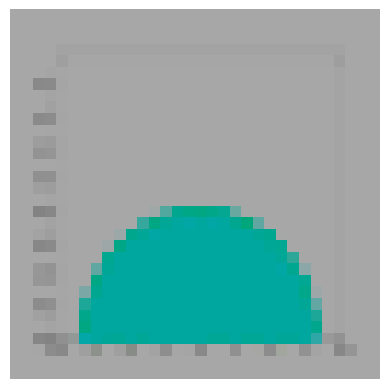
\includegraphics[width=\linewidth]{./img/color.png}
		\caption*{изменение свойств}
	\end{minipage}
	\caption{Пример изображений после преобразования.}
	\label{fig:transforms}
        \end{figure}


\end{frame}


\begin{frame}{Разработка приложения}

	\begin{alertblock}{Этапы разработки приложения}
            \begin{enumerate}
                \item Порождение изображений графиков вероятностных распределений;
                \item Применение аугментаций и необходимых преобразований над изображениями;
                \item Обучение нейронной сети на тренировочном наборе данных;
                \item Взаимодействие с нейронной сетью, получение предсказаний.
            \end{enumerate}
        \end{alertblock}

\end{frame}

\begin{frame}{Тестирование лучшей модели}

В результате исследования наилучшей моделью оказалась та, что была обучена на изображениях с изменёнными свойствами.

В результате тестирования выбранная модель правильно предсказала все классы сгенерированных изображений. На графиках, нарисованных от руки, модель правильно классифицировала три изображения из шести. 

\begin{figure}[H]
	\centering
	\begin{minipage}[t]{.45\textwidth}
		\centering
		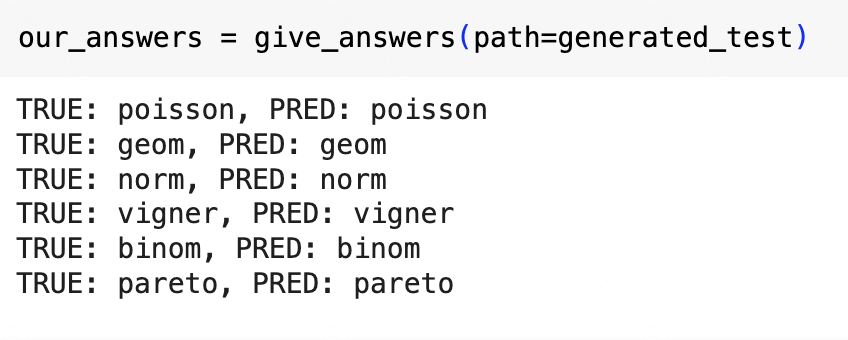
\includegraphics[width=0.7\linewidth]{./img/gen_res.png}
		\caption*{сгенерированные графики.}
	\end{minipage}
	\noindent
	\begin{minipage}[t]{.45\textwidth}
		\centering
		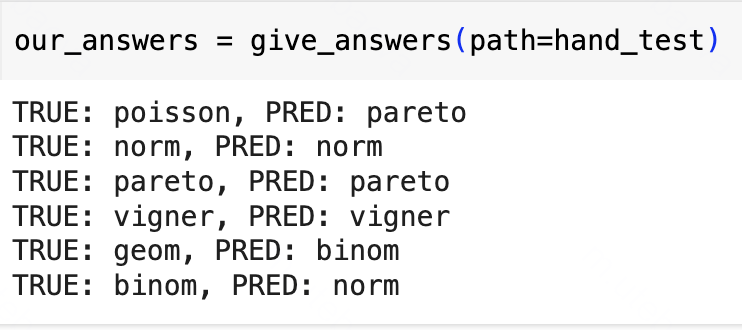
\includegraphics[width=0.7\linewidth]{./img/hand_res.png}
		\caption*{графики от руки.}
	\end{minipage}
	\caption{Результаты тестирования.}
	\label{fig:hand2}
\end{figure}

\end{frame}


\begin{frame}{Заключение}
  \begin{alertblock}{Возможные улучшения}
  \begin{itemize}
    \item Расширение набора тренировочных данных; 
    \item Улучшение архитектуры нейронной сети; 
    \item Дообучение нейронной сети на сложных примерах.
  \end{itemize}
  \end{alertblock}
\end{frame}

\begin{frame}{Заключение}
  В ходе разработки были получены следующие навыки:
    \begin{itemize}
      \item Разработка нейронных сетей и методов для взаимодействия с ними;
      \item Разработка функций для манипулирования изображениями;
      \item Использование разнообразных библиотек для исследований в области машинного обучения и анализа данных.
    \end{itemize}
\end{frame}



\end{document}